\section{Risultati e conclusioni}
\lhead{Risultati e conclusioni} % section header

Ogni  algoritmo, per stesso valore di budget \textit{k} e stessa funzione di costo \( c : V \rightarrow \mathbb{N} \) (e per stessa funzione submodulare \( f : 2^V \rightarrow \mathbb{R}^+ \), nel caso dell'algoritmo \textit{Cost-Seeds-Greedy}) è stato eseguito 10 volte. La sperimentazione è consistita nello studiare, al variare del budget \textit{k}, il numero medio di nodi influenzati (la taglia media dell'insieme \textit{Inf}) dal Seed-Set generato dall'algoritmo specificato, sulla funzione di costo specificata (e per la funzione submodulare specificata, nel caso dell'algoritmo \textit{Cost-Seeds-Greedy}).

Gli algoritmi utilizzati sono:
\begin{itemize}
  \item CSG (Cost Seeds Greedy)
  \item WTSS (Weighted Target Set Selection)
  \item My-Seeds (l'algoritmo ideato)
\end{itemize}

Le funzioni di costo \( c : V \rightarrow \mathbb{N} \) sono:

\begin{itemize}
  \item \(c(v) \sim U(1,10)\) 
  \item \(c(v) = \lceil \frac{d(v)}{2} \rceil\)
  \item \(c(v) = \lceil \frac{d(v)^2}{d_{\text{max}}} \rceil\)
\end{itemize}

Nel caso specifico dell'algoritmo Costs-Seeds-Greedy, le funzioni submodulari sono:

\begin{itemize}
  \item \(f_1(S) = \sum_{v \in V} \min\{|N(v) \cap S|, \lceil \frac{d(v)}{2} \rceil\}\) 
  \item \(
f_2(S) = \sum_{v \in V} \sum_{i=1}^{|N(v) \cap S|} \max\left\{\lceil \frac{d(v)}{2} - i + 1, 0 \right\}
\)
  \item \(
f_3(S) = \sum_{v \in V} \sum_{i=1}^{|N(v) \cap S|} \max\left\{\frac{\lceil \frac{d(v)}{2} - i + 1 \rceil}{d(v) - i + 1}, 0 \right\}
\)
\end{itemize}

\subsection{Risultati per Cost Seeds Greedy}

Nei seguenti grafici è possibile osservare, rispettivamente per la prima funzione submodulare, la seconda e la terza, la size media di \textit{Inf} al variare del budget \textit{k}, per le tre diverse funzioni di costo (i tre colori diversi). L'algoritmo utilizzato è Cost-Seeds-Greedy.

\begin{figure}[hbtp]
    \centering
    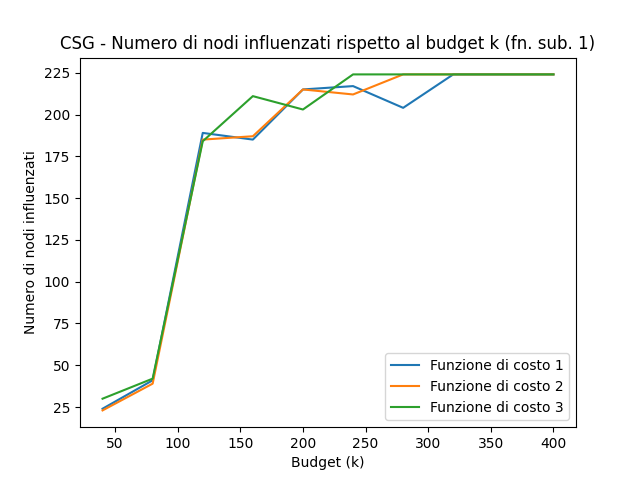
\includegraphics[width=0.75\textwidth]{images/csg_submodular_function_0.png}
    \caption*{Size media di Inf al variare di k (SF1)}
    \label{fig:first}
\end{figure}

\begin{figure}[hbtp]
    \centering
    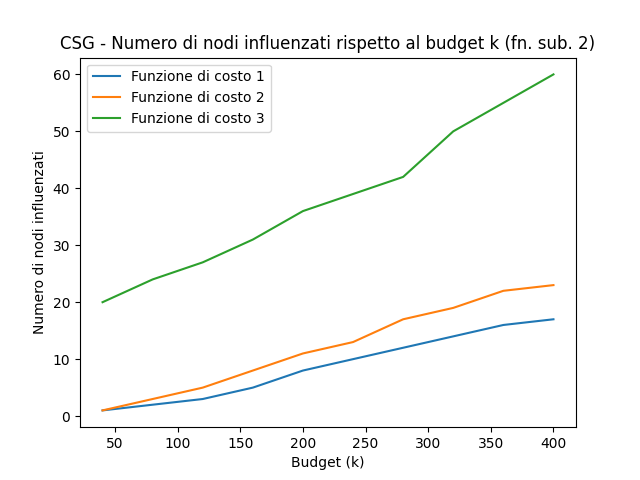
\includegraphics[width=0.75\textwidth]{images/csg_submodular_function_1.png}
    \caption*{Size media di Inf al variare di k (SF2)}
    \label{fig:second}
\end{figure}

\begin{figure}[hbtp]
    \centering
    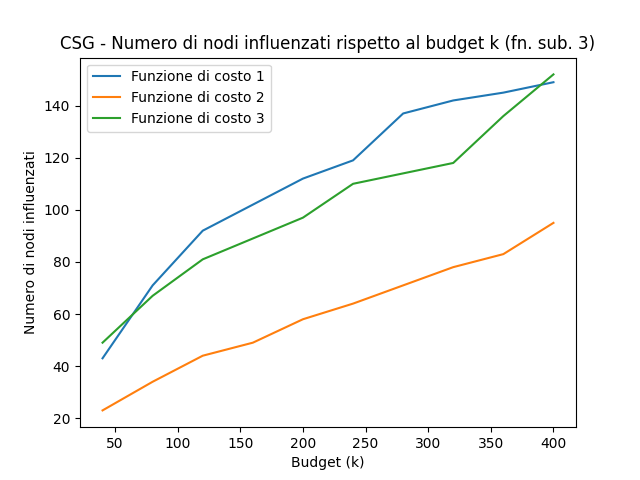
\includegraphics[width=0.8\textwidth]{images/csg_submodular_function_2.png}
    \caption*{Size media di Inf al variare di k (SF3)}
    \label{fig:third}
\end{figure}

È possibile osservare, per ogni funzione submodulare, per ogni funzione di costo utilizzata, un andamento pressochè crescente per ogni funzione. La size media dell'insieme dei nodi influenzati aumenta con l'aumentare del budget. 

I risultati migliori si ottengono con l'utilizzo della \textbf{prima funzione submodulare}, dove a prescindere alla funzione di costo, a partire da un budget di circa 300, il seed-set generato è in grado di raggiungere una complete cascade, influenzando tutti i nodi della rete.

I risultati peggiori sono ottenuti in corrispondenza dell'utilizzo della \textbf{seconda funzione submodulare} dove anche il budget massimo utilizzato per la sperimentazione (k = \textbf{400}) genera seed-sets in grado di influenzare in media circa \textbf{60} nodi (compresi i nodi appartenenti ai seed-set stessi), appena poco più del 25\% dei nodi totali della rete (\textbf{224} nodi).

I grafici relativi alle funzioni submodulari 2 e 3 condividono una \textbf{natura lineare}, aventi offset diversi a seconda della funzione di costo specificata e quasi tutte lo stesso coefficiente angolare.

Differente la \textbf{natura quasi logaritmica} presentata dalle funzioni di costo nella sperimentazione dove è fissata la funzione submodulare 1.


\subsection{Risultati per Weighted Target Set Selection}

Nel seguente grafico è possibile osservare la size media di \textit{Inf} al variare del budget \textit{k}, per le tre diverse funzioni di costo (i tre colori diversi). L'algoritmo utilizzato è Weighted Target Set Selection.

\begin{figure}[hbtp]
    \centering
    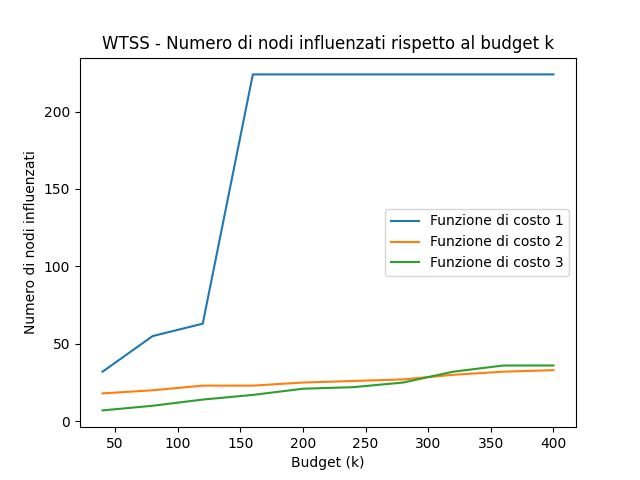
\includegraphics[width=0.75\textwidth]{images/wtss.png}
    \caption*{Size media di Inf al variare di k}
    \label{fig:third}
\end{figure}

È possibile osservare come, per lo stesso algoritmo WTSS, funzioni di costo diverse mostrano funzioni con comportamenti diversi. Tutte le funzioni hanno una natura crescente ma non lo stesso andamento; in particolare, per quanto riguarda la funzione di costo 1, in media è possibile raggiungere una complete cascade con un budget limitato, già a partire da k = \textbf{160} circa. 

Per la funzione 1 è possibile osservare un rapido incremento della size media di Inf a partire da budget appena più grandi di k = \textbf{140}, fenomeno che non è invece possibile osservare quando invece è utilizzata la seconda o la terza funzione di costo, che hanno un andamento lineare e non riescono ad influenzare più di 30 nodi anche avendo a disposizione il massimo budget (k = \textbf{400}).

\subsection{Risultati per MySeeds}

\begin{figure}[hbtp]
    \centering
    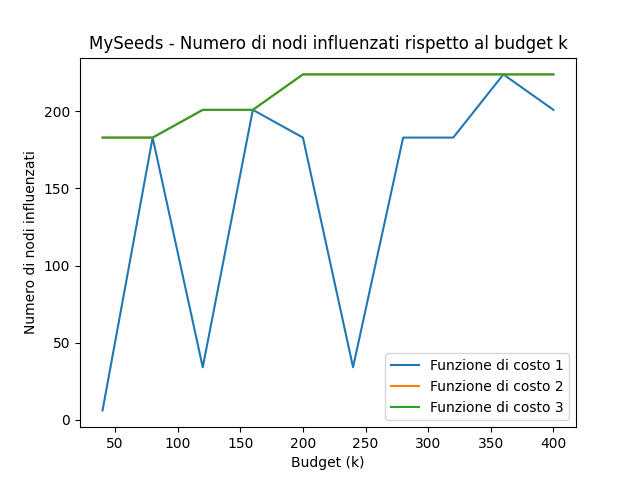
\includegraphics[width=0.75\textwidth]{images/custom.png}
    \caption*{Size media di Inf al variare di k}
    \label{fig:third}
\end{figure}

\vskip\baselineskip

Di seguito vengono allegati i grafici dei grafi generati tramite il processo di diffusione. In particolare, ogni riga rappresenta una tripletta di grafici in cui il primo grafico è una semplice rappresentaizone del grafo in cui i nodi sono colorati di grigio; il secondo grafico è una rappresentazione in cui i nodi afferenti al seed set (individuati mediante uno dei tre algoritmi considerati) è colorato in rosso, e i restanti nodi sono colorati in grigio; il terzo grafico è una rappresentazione in cui i nodi afferenti al seed set sono colorati in rosso, e i nodi influenzati ("Inf") dal seed set sono colorati in blu, mentre i restanti nodi sono colorati in grigio.

Queste rappresentazioni grafiche, di cui di seguito se ne rilascia solo una parte, mentre è possibile trovare ulteriori grafici sulla repository del progetto nella directory "graphs", permettono di capire quale configurazione riesce a raggiungere e quindi influenzare il maggior numero di nodi.

In particolare, si presentano grafici relativi a sperimentazioni legati alla rete 348, fissando la funzione di costo alla prima, e facendo variare il budget K (160, 320), e usando tutti gli algoritmi a disposizioni, per un totale di oltre 18 grafici. E' possibile produrre ulteriori grafici usando la CLI del programma, come descritto nelle sezioni precedenti.

Ad esempio, dai grafici è possibile osservare che l'algoritmo MySeeds performi nettamente meglio in un contesto ad alto budget, mentre gli algoritmi WTSS e CSG riescono in ogni caso a penetrare notevolmente la rete. Si nota che i grafici per K = 320 sono disponibili su GitHub.

\newpage

\begin{figure}[h]
  \centering
  \begin{subfigure}[b]{0.3\textwidth}
    \centering
    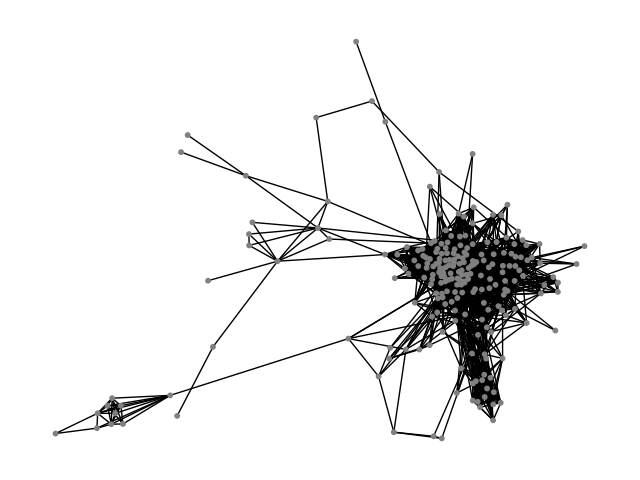
\includegraphics[width=\textwidth]{images/rete348_alg1_k160_cf1/pre-influencing.png}
    \caption{Rete 348, K=160, CF=1, Alg. CSG - Grafo di base}
    \label{fig:sub1}
  \end{subfigure}
  \hfill
  \begin{subfigure}[b]{0.3\textwidth}
    \centering
    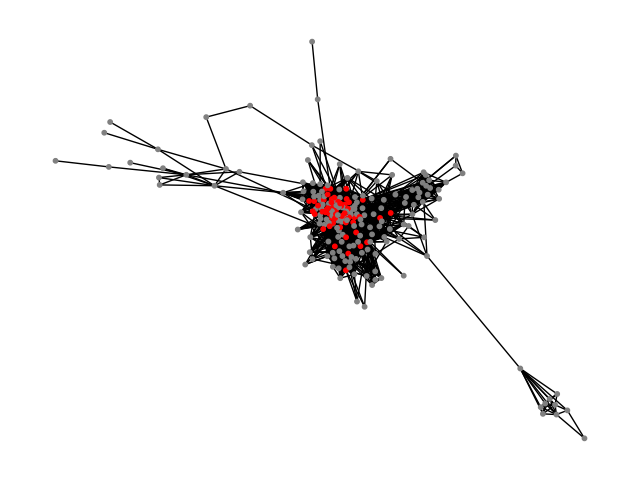
\includegraphics[width=\textwidth]{images/rete348_alg1_k160_cf1/influencing.png}
    \caption{Rete 348, K=160, CF=1, Alg. CSG - Seed Set}
    \label{fig:sub2}
  \end{subfigure}
  \hfill
  \begin{subfigure}[b]{0.3\textwidth}
    \centering
    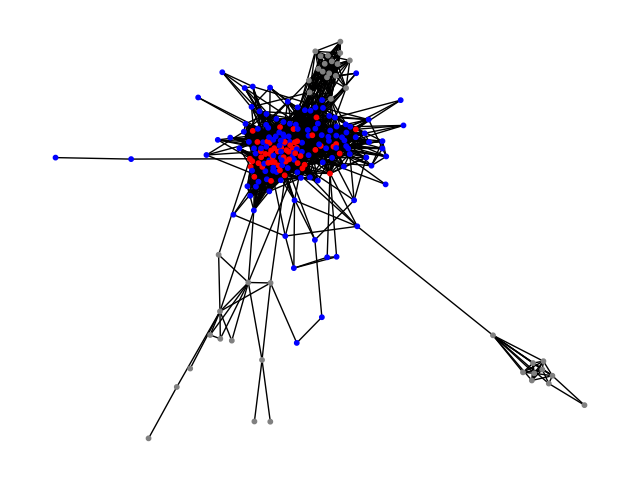
\includegraphics[width=\textwidth]{images/rete348_alg1_k160_cf1/influencing_and_influenced.png}
    \caption{Rete 348, K=160, CF=1, Alg. CSG - Seed Set \& Influenced}
    \label{fig:sub3}
  \end{subfigure}
  \label{fig:grid}
  \vskip\baselineskip
  \centering
  \begin{subfigure}[b]{0.3\textwidth}
    \centering
    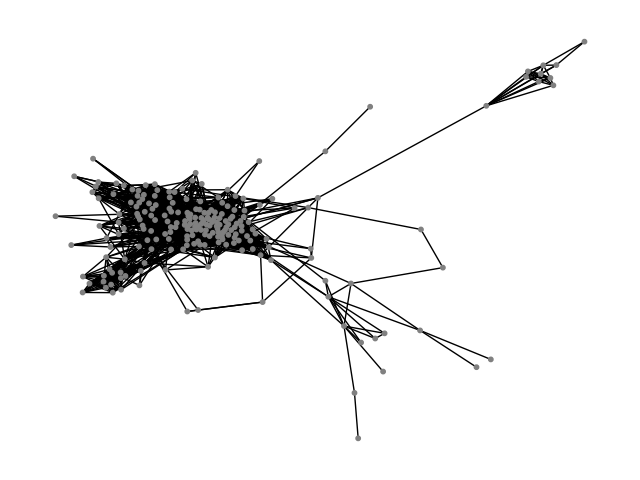
\includegraphics[width=\textwidth]{images/rete348_alg2_k160_cf1/pre-influencing.png}
    \caption{Rete 348, K=160, CF=1, Alg. WTSS - Grafo di base}
    \label{fig:sub1}
  \end{subfigure}
  \hfill
  \begin{subfigure}[b]{0.3\textwidth}
    \centering
    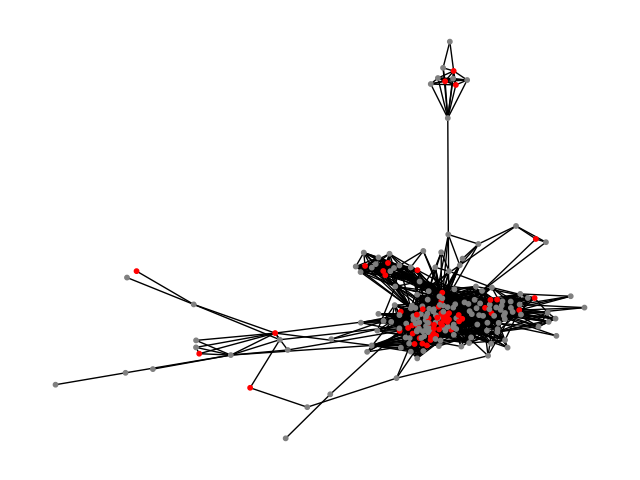
\includegraphics[width=\textwidth]{images/rete348_alg2_k160_cf1/influencing.png}
    \caption{Rete 348, K=160, CF=1, Alg. WTSS - Seed Set}
    \label{fig:sub2}
  \end{subfigure}
  \hfill
  \begin{subfigure}[b]{0.3\textwidth}
    \centering
    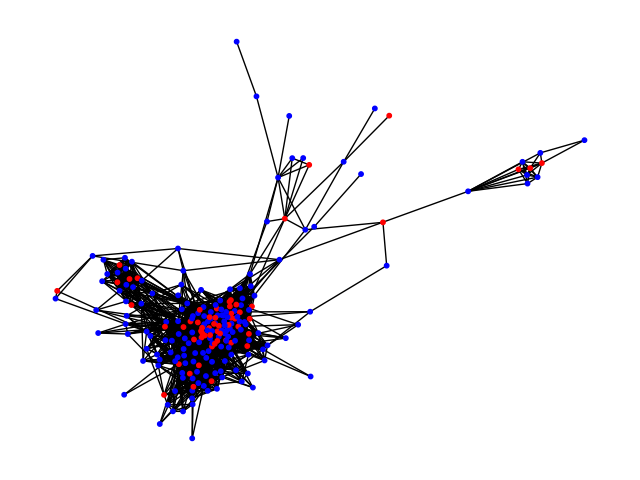
\includegraphics[width=\textwidth]{images/rete348_alg2_k160_cf1/influencing_and_influenced.png}
    \caption{Rete 348, K=160, CF=1, Alg. WTSS - Seed Set \& Influenced}
    \label{fig:sub2}
  \end{subfigure}
  \label{fig:grid}
  \vskip\baselineskip
  \centering
  \begin{subfigure}[b]{0.3\textwidth}
    \centering
    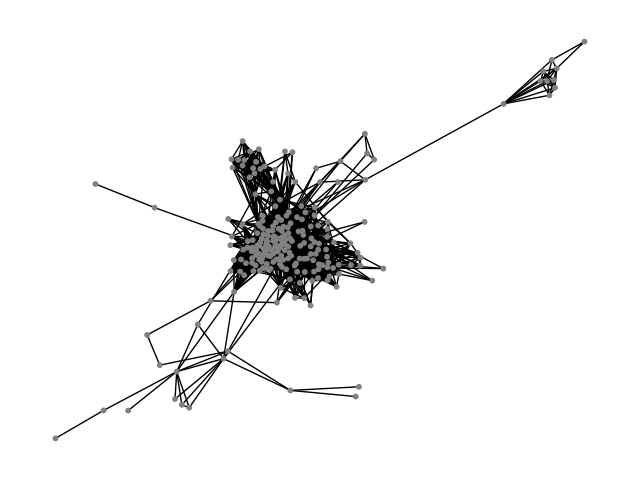
\includegraphics[width=\textwidth]{images/rete348_alg3_k160_cf1/pre-influencing.png}
    \caption{Rete 348, K=160, CF=1, Alg. MySeeds - Grafo di base}
    \label{fig:sub1}
  \end{subfigure}
  \hfill
  \begin{subfigure}[b]{0.3\textwidth}
    \centering
    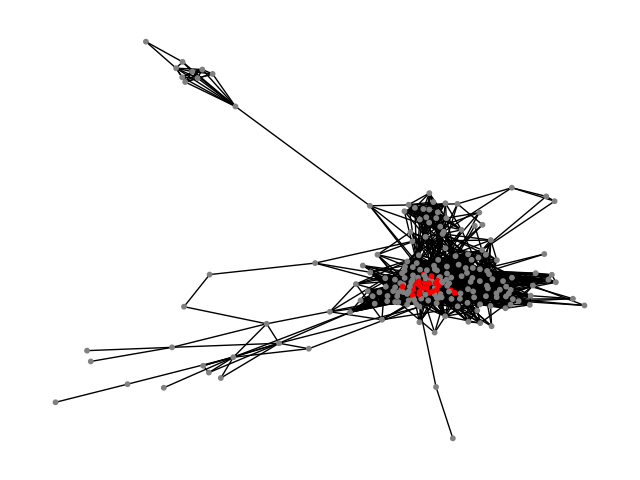
\includegraphics[width=\textwidth]{images/rete348_alg3_k160_cf1/influencing.png}
    \caption{Rete 348, K=160, CF=1, Alg. MySeeds - Seed Set}
    \label{fig:sub2}
  \end{subfigure}
  \hfill
  \begin{subfigure}[b]{0.3\textwidth}
    \centering
    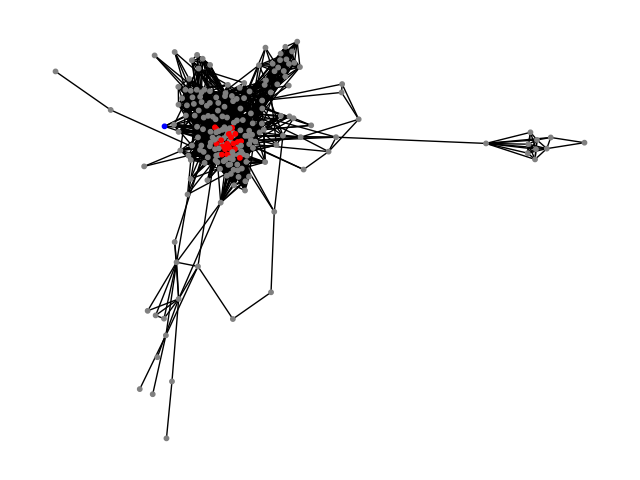
\includegraphics[width=\textwidth]{images/rete348_alg3_k160_cf1/influencing_and_influenced.png}
    \caption{Rete 348, K=160, CF=1, Alg. MySeeds - Seed Set \& Influenced}
    \label{fig:sub2}
  \end{subfigure}
\end{figure}

\newpage